%%%%%%%%%%%%%%%%%%%%%%%%%%%%%%%%%%%%%%%%%%%%%%%%%%%%%%%%%%%%%%%%%%%%%%%
%      SEC. 1
%%%%%%%%%%%%%%%%%%%%%%%%%%%%%%%%%%%%%%%%%%%%%%%%%%%%%%%%%%%%%%%%%%%%%%%
\section{Introduction and structure of the thesis}

Passion and curiosity should always lie at the heart of the scientific practice, and that ought to be enough to define the value of a research effort~\cite{Weber1917,Shapin2015}. Time is the real arbiter of the significance of a piece of research, as many examples in the history of science show~\cite{Brush1967,Niss2008}\footnote{The Ising-Lenz model is one such example~\cite{Brush1967,Niss2008,Niss2004}. It was suggested by physicist Wilhelm Lenz to his doctoral student Ernst Ising to study phase transitions in ferromagnetic materials. Ising solved it analytically in 1D as part of his Ph.D. defense in 1925, but the solution for a 1D lattice did not show any phase transition. This apparent failure is thought to be the reason of Ising's decision to take a job outside academia. Almost 20 years later, Onsager solved the 2D version of the model and showed the possibility of phase transitions in the Ising-Lenz model. By the time Ising arrived in the USA in 1947, the Ising-Lenz model was already entering the canon of physics and, to his surprise, he was being asked if he was ``the Ising" of the ``Ising model".}.However, in these years of increasing mistrust towards scientific research and brewing doubts on the value of universities and research institutes~\cite{Biesta2002,Biesta2004,Santos2012}, it is worthwhile to try to place one's own work into the wider picture of one's own time. It is also a valuable exercise for the researcher, who sensibly progresses in the work by investigating one detail at a time, to spend a moment away from one's own graphs and equations and see their place in the wider perspective of the world outside the laboratory.\\
It is thus in this spirit that I propose to open the present work with a reflection on the challenges that the transportation industry faces at the closing of $21^{st}$ century's second decade. Against this background, in Chapter~1 \emph{thin-ply} laminates are introduced as a very promising material for innovative structural design and their main characteristics are discussed. The focus is then moved to the most renown quality of \emph{thin-ply} laminates, i.e. their ability to delay and even suppress onset and propagation of transverse cracking, and to discuss the modeling issues that this new material poses. Finally, a link is established with the growth of fiber/matrix interface cracks or, as very often called in the rest of the thesis, debonds. Chapter~2 opens with an introduction to the main concepts of Fracture Mechanics. The fiber/matrix interface crack is then discussed in detail, and previous analytical, computational and experimental studies available in the literature are reviewed. The modeling strategy adopted in this thesis is then presented and its implementation described. Finally, Chapter~3 provides a summary of the main results of this work, organized following the order of the publications reported in Part~II of the thesis. The first chapter is thus a journey of scales: we start from the challenges of an industrial sector, move to the structural requirements of its products, focus on a promising new material, and concentrate on understanding the mechanisms of damage initiation in it.

\section{Vision 2030: challenges of the next decade and beyond for the transportation industry}

The closing of the second decade of the $21^{st}$ century brings different challenges for the transportation industry, which will likely shape its development in the next decade and beyond. A brief review of the most relevant aspects is proposed here.

\begin{description}
\item[Climate action.] The issue of climate change is certainly one the ``hot" topic of today's public debate. A discussion of the merits of scientific understanding of climate change, public reception, media coverage and socio-political implications is out of the scope of the present work, but it is certainly one of the most relevant topic framing today's public discourse. Given that it is a high-divisive subject, no judgement on the validity of the claims of one side or the other is proposed here, as sufficient space can not be devoted to a thorough analysis of the problem. What is acknowledged here is the emergence of concerted efforts at the institutional level (companies, city administrations, regional governments, sovereign states) to rule into and provide control mechanisms to limit the emission of carbon dioxide, i.e. $CO_{2}$. The evidence of this shift in public policy is exemplified in Figure~\ref{chap1:fig:climatedealssignataries} and Figure~\ref{chap1:fig:greenfundpledges}.\\ Figure~\ref{chap1:fig:climatedealssignataries} reports the evolution over time of the number of signatories of three representative deals on climate action. The selected deals are: the Vienna Convention for the Protection of the Ozone Layer, first signed in 1985 and committing signatories to the reduction of chlorofluorocarbons; the United Nations Framework Convention on Climate Change (UNFCCC), initially agreed in 1992 with the aim of managing the increase in greenhouse emission in order to avoid dangerous interferences with the climate; the Kyoto Protocol, signed in 1997 as an extension of the UNFCCC and according to which adhering countries pledge to reduce greenhouse emissions to prevent climate change. Figure~\ref{chap1:fig:climatedealssignataries} shows how the majority of countries have ratified these deals over time, reaching an almost unanimous agreement on the need of coordinated action towards the issues of climate change.

\begin{figure}
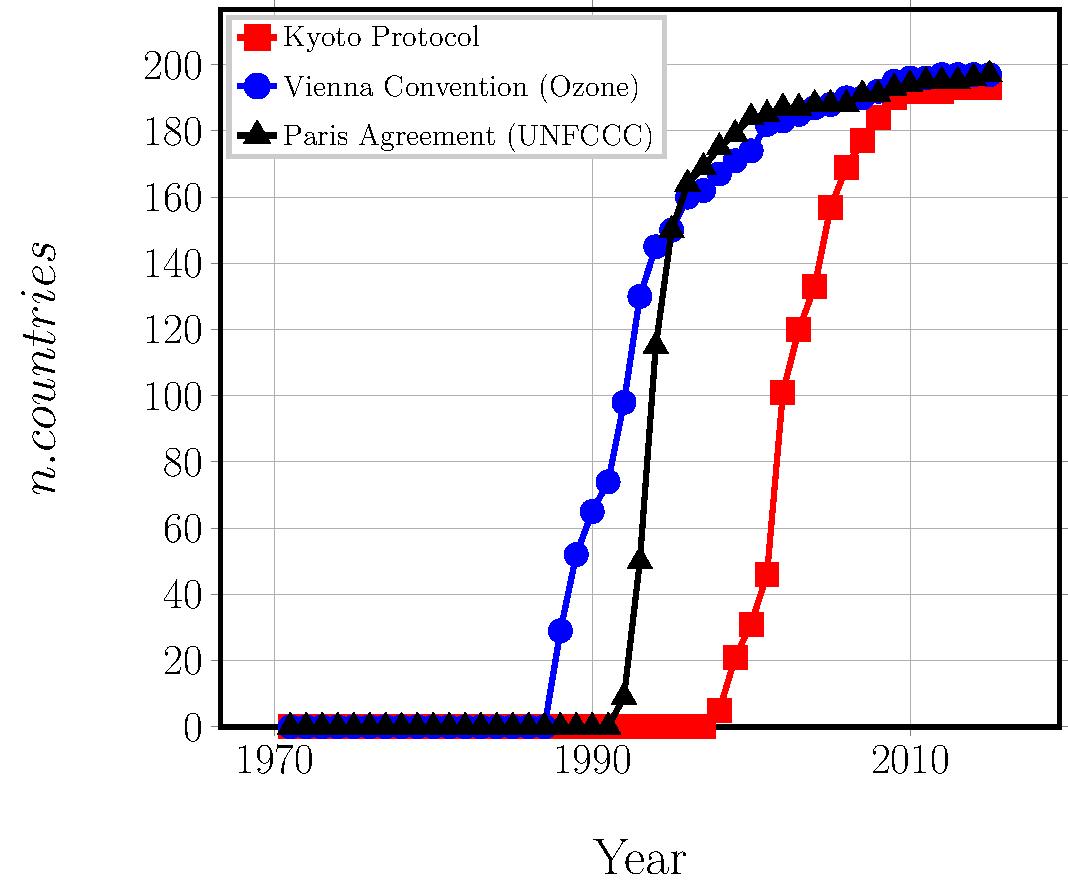
\includegraphics[width=\textwidth]{pics/climate-deals-signataries.pdf}
\caption{Number of signing countries over time for selected deals on climate. Source: UNCTAD Development and Globalization: Facts and Figures (2016). United Nations Conference on Trade and Development. Available at \href{https://stats.unctad.org/Dgff2016/DGFF2016.pdf}{https://stats.unctad.org/Dgff2016/DGFF2016.pdf} (last access: September 26, 2019).}\label{chap1:fig:climatedealssignataries}
\end{figure}

Figure~\ref{chap1:fig:greenfundpledges} shows the 10 highest contributions to the Green Climate Fund, which aims to support projects in developing countries focusing on reduction of greenhouse gas emissions and climate adaptation. The commitment to this effort of industrialized countries is evident in Figure~\ref{chap1:fig:greenfundpledges}.

\begin{figure}
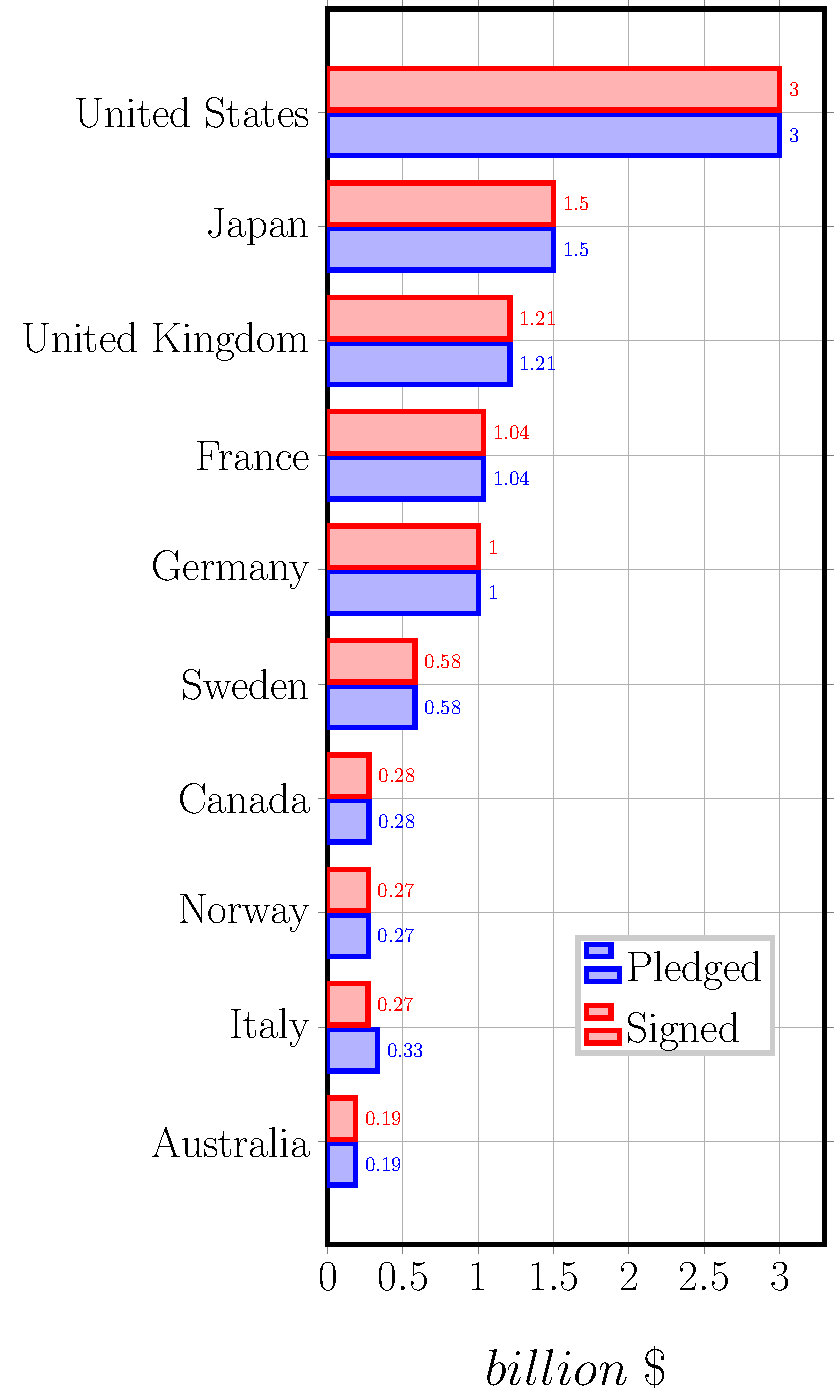
\includegraphics[height=\textheight]{pics/green-fund-pledges.pdf}
\caption{Pledged and signed contributions to the Green Climate Fund of the 10 countries with the highest signed contributions. Source: Green Climate Fund, available at \href{https://www.greenclimate.fund/how-we-work/resource-mobilization}{https://www.greenclimate.fund/how-we-work/resource-mobilization} (last access: September 21, 2019).}\label{chap1:fig:greenfundpledges}
\end{figure}

Some relevant data is also presented in order to show the importance of the issue for the transportation industry.

\begin{figure}
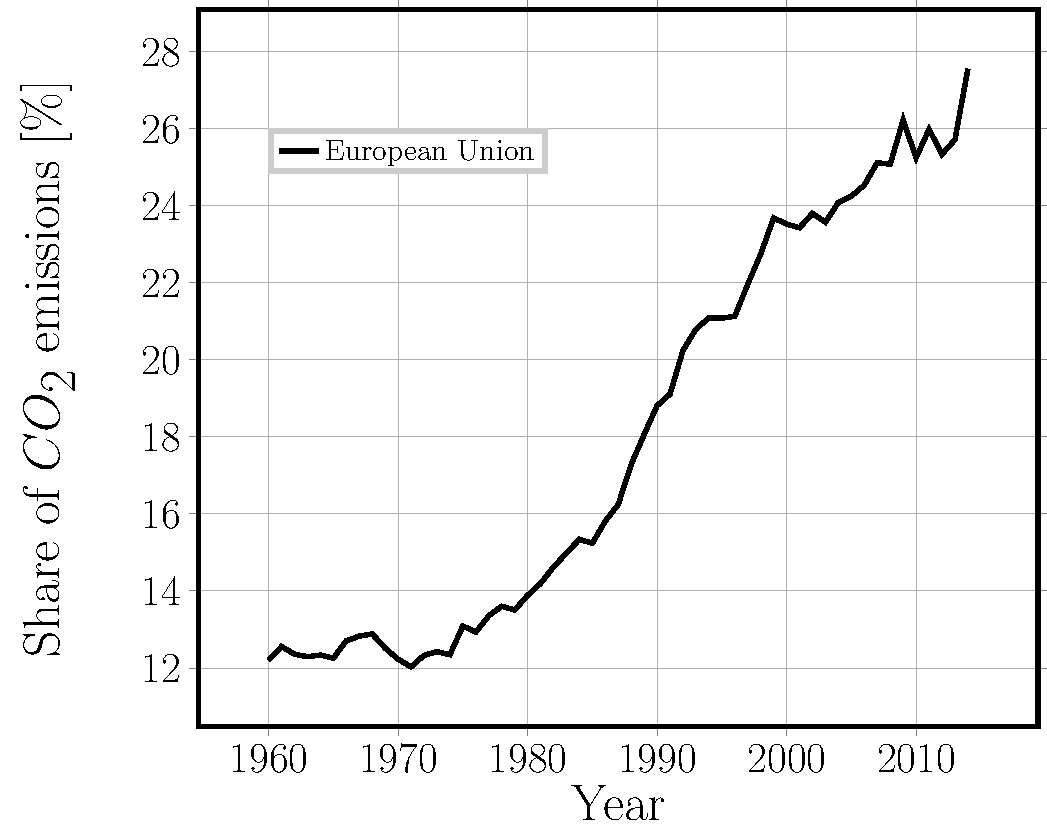
\includegraphics[width=\textwidth]{pics/co2transportshare.pdf}
\caption{Share of total $CO_{2}$ emissions due to the transport sector over time for selected countries. Source: International Energy Agency (IEA) via The World Bank, available at \href{http://data.worldbank.org/data-catalog/world-development-indicators}{http://data.worldbank.org/data-catalog/world-development-indicators} (last access: September 21, 2019).}\label{chap1:fig:co2transportshare}
\end{figure}

\begin{figure}
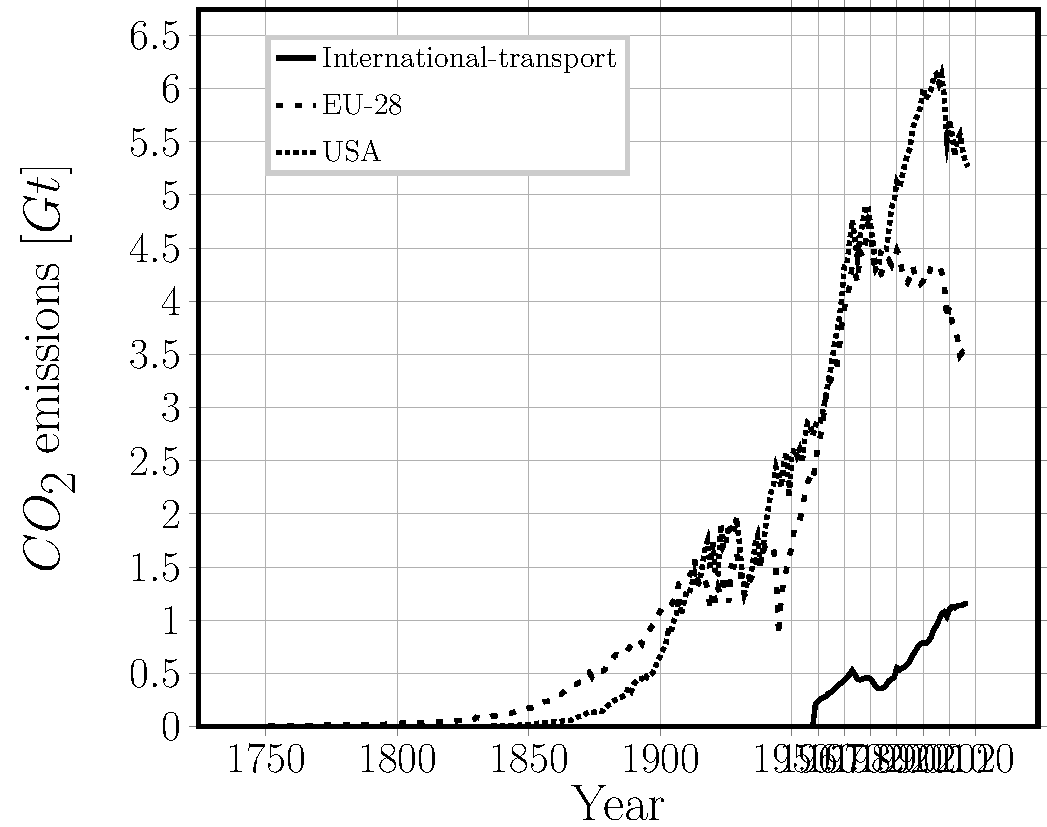
\includegraphics[width=\textwidth]{pics/co2transportabsolute.pdf}
\caption{Total $CO_{2}$ emissions due to transport over time, compared with selected geographical entities. Source: The Global Carbon Project, available at \href{https://www.globalcarbonproject.org/}{https://www.globalcarbonproject.org/} (last access: September 21, 2019).}\label{chap1:fig:co2transportabsolute}
\end{figure}

\end{description}
